% ===================== CAPA PERSONALIZADA =====================
\definecolor{capaline}{HTML}{29797c} % identidade visual UFCAT
\newcommand{\CapaLinha}{\noindent\begingroup
  \color{capaline}\rule{\textwidth}{5pt}
\endgroup}

\newcommand{\CapafontXVI}{\bfseries\fontsize{16pt}{24pt}\selectfont}
\newcommand{\CapafontXVIII}{\fontsize{18pt}{27pt}\selectfont}
% tamanhos pedidos para o cabeçalho visual da capa
\newcommand{\CapafontXXXVI}{\bfseries\fontsize{36pt}{54pt}\selectfont} % 36 pt (bold)
\newcommand{\CapafontXIV}{\fontsize{14pt}{21pt}\selectfont}            % 14 pt

\newcommand{\capaSigla}{UFCAT}
\newcommand{\capaNome}{Universidade Federal de Catalão}
\newcommand{\capalogo}{template_eca_ufsc_abnt/figuras/identidade_visual.png}


\makeatletter
\newcommand{\capadata}{
CATALÃO

2025/2}
\makeatother

% NÃO usar page style na capa (evita vazamentos no topo)

\renewcommand{\imprimircapa}{%
  \begin{titlepage}
    % Sem cabeçalho/rodapé na capa: some “1.5 1.5”
    \thispagestyle{empty}

    \renewcommand{\ABNTEXchapterheadstartvskip}{\vspace*{-2cm}}

    % Topo da capa — UFCAT 36pt / Universidade 14pt — isolado do 1,5 global
    \begingroup
      %\setstretch{1.1}
      % ajuste fino do topo (negativo sobe, positivo desce):
      \vspace*{-3.5cm}
      \begin{center}
        {\CapafontXXXVI UFCAT\par}
        {\CapafontXIV Universidade Federal de Catalão\par}
      \end{center}
    \endgroup

    % linha de identidade visual
    %\vspace*{0.5ex}
    %\CapaLinha

    % Miolo da capa
    \vspace*{40ex}
    \noindent{{\bfseries\fontsize{16pt}{16pt}\selectfont \MakeUppercase{\imprimirautor}}\par}

    \vspace*{0.5ex}
    \CapaLinha

% Título  
\vspace*{0.5ex}
    \noindent{\CapafontXVI \MakeUppercase{\imprimirtitulo}\par}

%Tipo de trabalho
\CapaLinha
\vspace*{0.5ex} 
    \noindent{\CapafontXVI \MakeUppercase{Trabalho de Conclusão de Curso}\par}

    \vfill
    \noindent
    \begin{minipage}[t]{0.5\textwidth}
      \includegraphics[height=3.34cm]{\capalogo}
    \end{minipage}%
    \begin{minipage}[t]{0.5\textwidth}
      \raggedleft
      {\CapafontXVIII \capadata}
    \end{minipage}
  \end{titlepage}
}

% Capa
\imprimircapa

% Folha de rosto
% o * indica que haverá a ficha bibliográfica
\imprimirfolhaderosto*

% % Inserir a ficha bibliografica
% % http://ficha.bu.ufsc.br/
% \begin{fichacatalografica}
% 	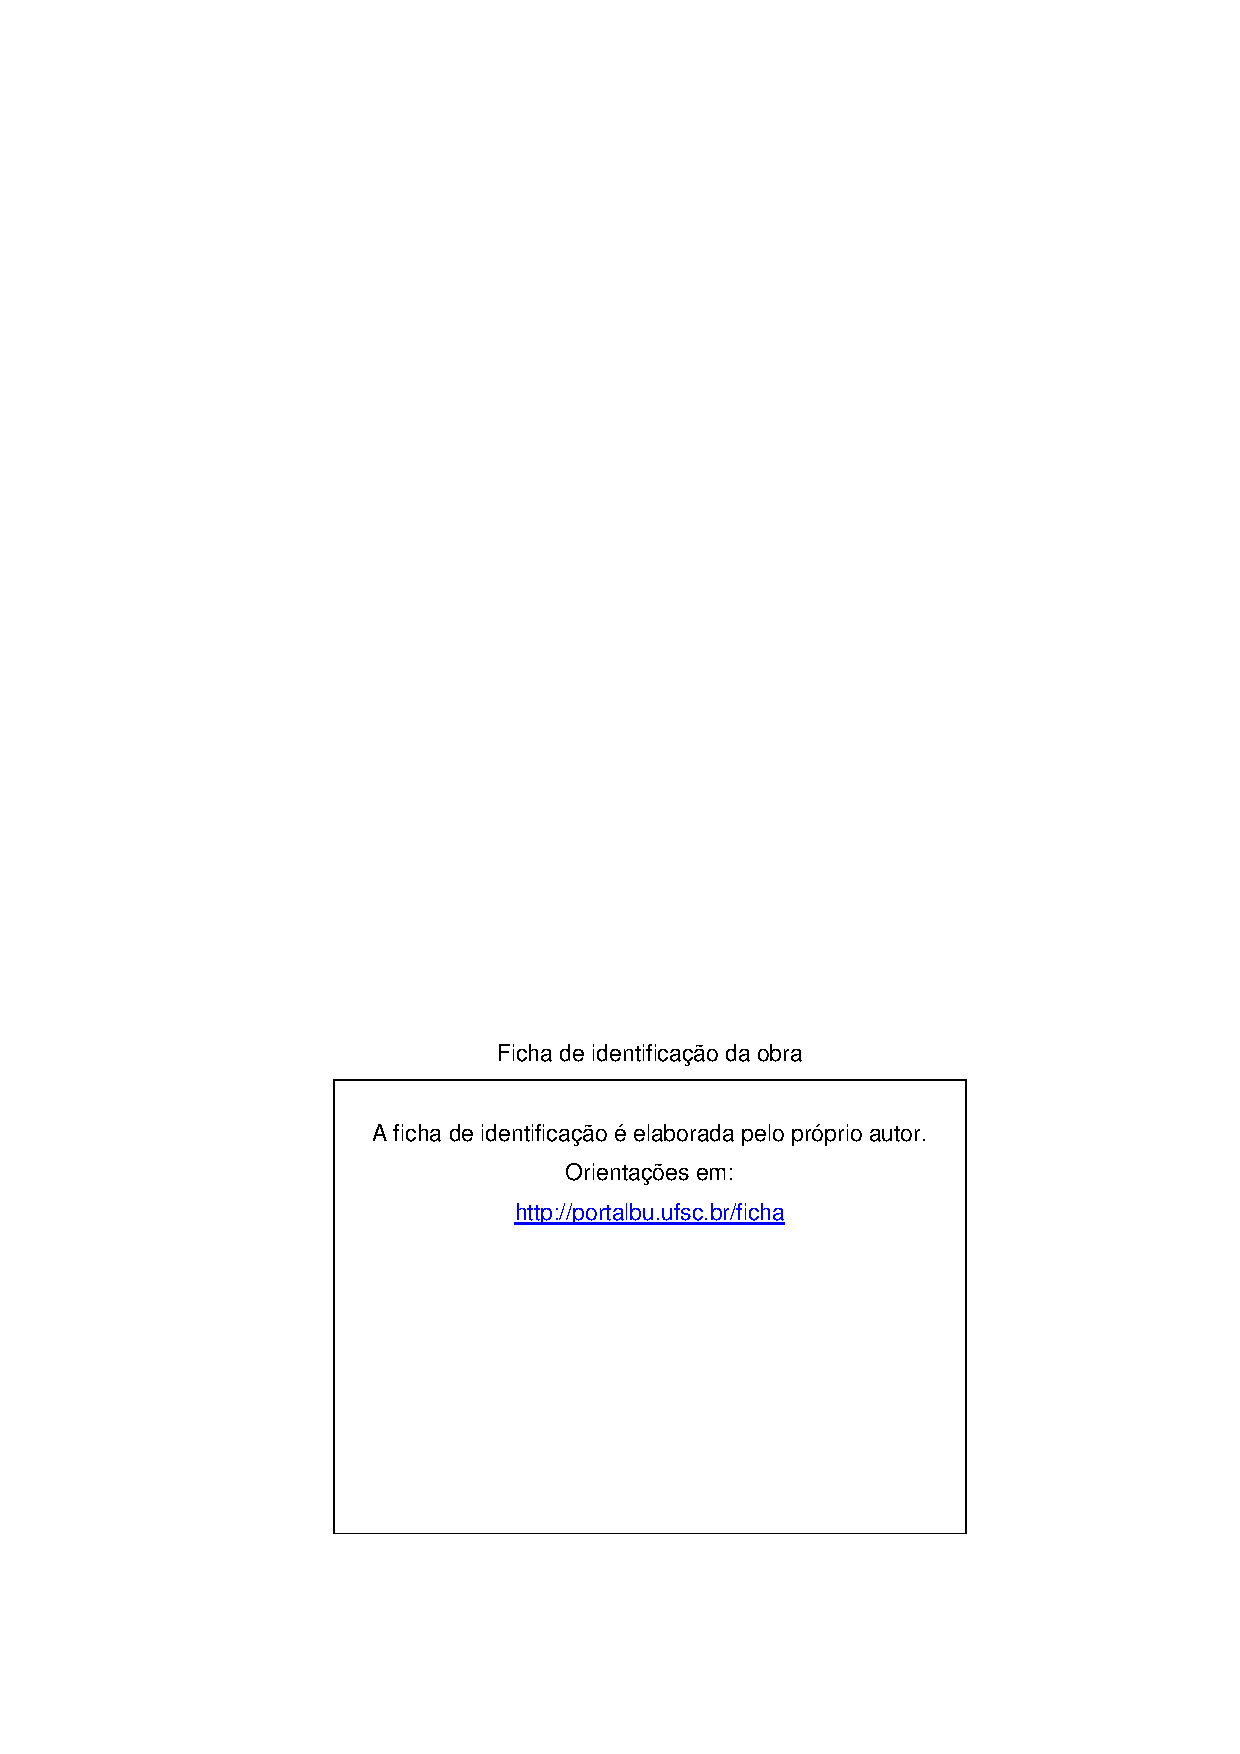
\includepdf{pre_textual/ficha_catalografica.pdf}
% \end{fichacatalografica}

% Inserir folha de aprovação
% \begin{folhadeaprovacao}
% 	\OnehalfSpacing
% 	\centering
% 	\imprimirautor\\%
% 	\vspace{24pt}		
% 	\textbf{\imprimirtitulo}%
% 	\ifnotempty{\imprimirsubtitulo}{:~\imprimirsubtitulo}\\%
% 	%		\vspace*{31.5pt}%3\baselineskip
% 	\vspace*{\baselineskip}
% 	%\begin{minipage}{\textwidth}
% 	Este Trabalho de Conclusão de Curso foi julgado adequado para obtenção do Título de ``\imprimirformacao'' e aprovado em sua forma final pelo Curso de Graduação em Engenharia Civil.\\
% 	\vspace{12pt}
% 	\imprimirlocal, \imprimirdia~de~\imprimirmes~de~\imprimirano.\\
	
% 	\vspace*{18pt}
% 	\textbf{Banca Examinadora:}\\
	
% 	\vspace*{24pt}
% 	\assinatura{\OnehalfSpacing \imprimirbancanomea}
% 	\vspace{6pt}
% 	\imprimirbancainsta\\
	
% 	\vspace*{24pt}
% 	\assinatura{\OnehalfSpacing \imprimirbancanomeb}
% 	\vspace{6pt}
% 	\imprimirbancainstb\\
	
% \end{folhadeaprovacao}

% ================== FOLHA DE APROVAÇÃO (AUTOMATIZADA) ==================
\begin{folhadeaprovacao}
    \thispagestyle{empty}
    \OnehalfSpacing

    \begin{center}
        % Puxa o autor do main
        {\fontsize{12pt}{12pt}\selectfont\MakeUppercase{\imprimirautor}\par}
        
        \vspace{15ex} 

        % Puxa o título do main
        {\fontsize{12pt}{12pt}\selectfont\bfseries\MakeUppercase{\imprimirtitulo}\par}
    \end{center}

    \vspace{10ex}

    % Preâmbulo alinhado à direita
    
    \begin{flushright}
        \begin{minipage}{0.5\textwidth}
            {\fontsize{11pt}{11pt}\selectfont
            Trabalho de Conclusão de Curso apresentado ao Curso de Engenharia Civil da Faculdade de Engenharia da Universidade Federal de Catalão como parte dos requisitos para obtenção do título de Bacharel em Engenharia Civil.\par}
        \end{minipage}
    \end{flushright}

    \vspace{10ex}


    \vspace{8ex}

    % Membros da Banca fazendo referência aos comandos do preâmbulo
    \begin{flushleft}
        {\fontsize{12pt}{12pt}\selectfont
        
        % Orientador (Geralmente definido como imprimirorientador)
        \imprimirorientador \\
        Orientador -- FENG/UFCAT \\
        \vspace{6ex}
        
        % Coorientador (Se houver)
        \ifnotempty{\imprimircoorientador}{
            \imprimircoorientador \\
            Coorientador -- FENG/UFCAT \\
            \vspace{6ex}
        }
        
        % Primeiro Membro da Banca (Wanderson Ferreira)
        \imprimirbancanomea \\
        Membro da Banca -- \imprimirbancainsta \\
        \vspace{6ex}
        
        % Segundo Membro da Banca (Romes Antonio)
        \imprimirbancanomeb \\
        Membro da Banca -- \imprimirbancainstb \par}
    \end{flushleft}

\end{folhadeaprovacao}

% Dedicatória
% \ifnotempty{\imprimirdedicatoriatcc}{
% \begin{dedicatoria}
% 	\vspace*{\fill}
% 	\noindent
% 	\begin{adjustwidth*}{}{7.5cm} 
% 		\textit{\imprimirdedicatoriatcc}
% 	\end{adjustwidth*}
% \end{dedicatoria}
% }
\ifnotempty{\imprimirdedicatoriatcc}{
\begin{dedicatoria}
    \vspace*{\fill}
    \begin{flushright}
        \begin{minipage}{0.5\textwidth}
            \itshape
            \imprimirdedicatoriatcc
        \end{minipage}
    \end{flushright}
\end{dedicatoria}
}

% Agradecimentos
\ifnotempty{\imprimiragradecimentostcc}{
\begin{agradecimentos}
	\imprimiragradecimentostcc
\end{agradecimentos}
}

% Epígrafe
% \ifnotempty{\imprimirepigrafetcc}{
% \begin{epigrafe}
% 	\vspace*{\fill}
%         \noindent
% 	\begin{adjustwidth*}{}{7.5cm}
%         \textit{\imprimirepigrafetcc}
%         \end{adjustwidth*}
% \end{epigrafe}
% }
\ifnotempty{\imprimirepigrafetcc}{
\begin{epigrafe}
    \vspace*{\fill}
    \begin{flushright}
        \begin{minipage}{0.5\textwidth}
            \itshape
            \imprimirepigrafetcc
        \end{minipage}
    \end{flushright}
\end{epigrafe}
}

% Resumo
\setlength{\absparsep}{18pt} % ajusta o espaçamento dos parágrafos do resumo
\begin{resumo}
	\OnehalfSpacing
	\imprimirresumotcc
	
	\textbf{Palavras-chave}: \imprimirpalavraschave
\end{resumo}

% Abstract
\begin{resumo}[Abstract]
	\OnehalfSpacing
	\imprimirabstracttcc
		
	\textbf{Keywords}: \imprimirkeywords
\end{resumo}

% % Inserir publicações. Caso não deseje informa comentar todo esse bloco de código
% \begin{folhadeaprovacao}

% \cleardoublepage
% \begin{center}
%   {\textbf{PUBLICAÇÕES \textcolor{red}{Está página é opcional}}}
% \end{center}
% Esta dissertação é baseada no(s) artigo(s) científico(s) publicado(s) na(s) seguinte(s) revista(s):
% \vspace{1em}
% \begin{itemize}
%   \item SANTIAGO, Wagner Carvalho; KROETZ, Henrique Machado; SANTOS, Sérgio Hampshire de C.; STUCCHI, Fernando Rebouças; BECK, André Teófilo. Reliability-based calibration of main Brazilian structural design codes. \textbf{Latin American Journal of Solids and Structure}s, v. 17, e245, fev. 2020.
% \end{itemize}
% \cleardoublepage

% \end{folhadeaprovacao}

{%hidelinks
	\hypersetup{hidelinks}
	
	% inserir lista de figuras
% {
% \SingleSpacing
% \pdfbookmark[0]{\listfigurename}{lof}
% \listoffigures*
% \cleardoublepage
% }
	
% % Lista de quadros
% {
% \SingleSpacing
% \ifnotempty{\verificaquadros}{
% \pdfbookmark[0]{\listofquadrosname}{loq}
% \listofquadros*
% \cleardoublepage
% }
	
% 	% inserir lista de tabelas

% {
% \SingleSpacing
% \pdfbookmark[0]{\listtablename}{lot}
% \listoftables*
% \cleardoublepage
% }
% 	% inserir lista de abreviaturas e siglas (devem ser declarados no preambulo)
% \ifnotempty{\verificasiglas}{
% \imprimirlistadesiglas
% }

% % inserir lista de símbolos
% \ifnotempty{\verificasimbolos}{
% \imprimirlistadesimbolos
% }

% % inserir o sumario
% \pdfbookmark[0]{\contentsname}{toc}
% \tableofcontents*
% \cleardoublepage
	
% }%hidelinks

% --- LISTA DE FIGURAS (Espaçamento Simples) ---
{
    \SingleSpacing 
    \pdfbookmark[0]{\listfigurename}{lof}
    \listoffigures*
    \cleardoublepage
}

% --- LISTA DE QUADROS (Espaçamento Simples) ---
\ifnotempty{\verificaquadros}{
    {
        \SingleSpacing
        \pdfbookmark[0]{\listofquadrosname}{loq}
        \listofquadros*
        \cleardoublepage
    }
}

% --- LISTA DE TABELAS (Espaçamento Simples) ---
{
    \SingleSpacing
    \pdfbookmark[0]{\listtablename}{lot}
    \listoftables*
    \cleardoublepage
}

% --- LISTA DE SIGLAS E ABREVIATURAS (Espaçamento 1.5) ---
\ifnotempty{\verificasiglas}{
    {
        \OnehalfSpacing
        \imprimirlistadesiglas
        \cleardoublepage
    }
}

% --- LISTA DE SÍMBOLOS (Espaçamento 1.5) ---
\ifnotempty{\verificasimbolos}{
    {
        \OnehalfSpacing
        \imprimirlistadesimbolos
        \cleardoublepage
    }
}


% --- SUMÁRIO DEFINITIVO (AJUSTE NÍVEL 0 E REMOÇÃO NÍVEL 4) ---
{
    \hypersetup{hidelinks}
    \pdfbookmark[0]{\contentsname}{toc}
    
    % Força o limite de profundidade (Subsection é o limite)
    \setcounter{tocdepth}{2}
    \setcounter{secnumdepth}{2}

    \makeatletter

    % --- AJUSTE RADICAL DO NÍVEL 0 (Chapter) ---
    % Esse comando remove o espaço elástico que o abntex2 coloca após o número
    \renewcommand{\cftchapteraftersnum}{\hspace{0em}} % Ajuste este valor (ex: 0.3em para mais perto)
    \setlength{\cftchapterindent}{0pt}
    \setlength{\cftchapternumwidth}{0.5em} % Espaço reservado para o número

    % --- NÍVEL 1 (Section) ---
    % Mantendo a escada: deve ser igual ao numwidth acima
    \setlength{\cftsectionindent}{1.2em} 
    \setlength{\cftsectionnumwidth}{2.0em}

    % --- NÍVEL 2 (Subsection) ---
    % Soma dos anteriores (1.2 + 2.0 = 3.2em)
    \setlength{\cftsubsectionindent}{3.2em}
    \setlength{\cftsubsectionnumwidth}{2.8em}

    % --- COMANDO PARA SUMIR COM O NÍVEL 4 ---
    % Se o tocdepth falhar, isso aqui deleta a subsubsection do sumário
    \expandafter\def\csname l@subsubsection\endcsname#1#2{}

    \makeatother

    \tableofcontents*
    \cleardoublepage
    \end{spacing} 
}